%Describe the experiments you conducted to evaluate the approach.  For each
%experiment, describe what you did, what was the main purpose of the experiment,
%and what you learned from the results. Provide figures, tables, and qualitative
%examples, as appropriate.

In this section, we evaluate our method on the MIT-indoor67 dataset. Suggested training and
testing list of images are used to do the training (80 images per class) and validation (20
images per class), all images are in jpeg format. We notice that several
pairs of categories are relatively easier to be confused and misclassified by the
SVMs with each other (For the detaled confusion matrix, please refer to Figure~\ref{fig:confusion_matrix} in the Appendix. Such examples include bakery and deli, living room and bedroom, as well as
bookstore and library. We show some sample training and testing images from these
pairs in Figure~\ref{fig:sample}. For the bakery and deli pair, they both contain very
similar patterns of breads and sandwiches on shelves. For the livingroom and bedroom
pair, some living room images may include bed or bed-like sofa, which is almost identical
to the beds and sofas in images from bedroom category. For the library and bookstore,
both contain identical shelves of books. It is very difficult, even for human beings, to distinguish
images between these two categories.

\begin{figure}[ht]
  \centering
  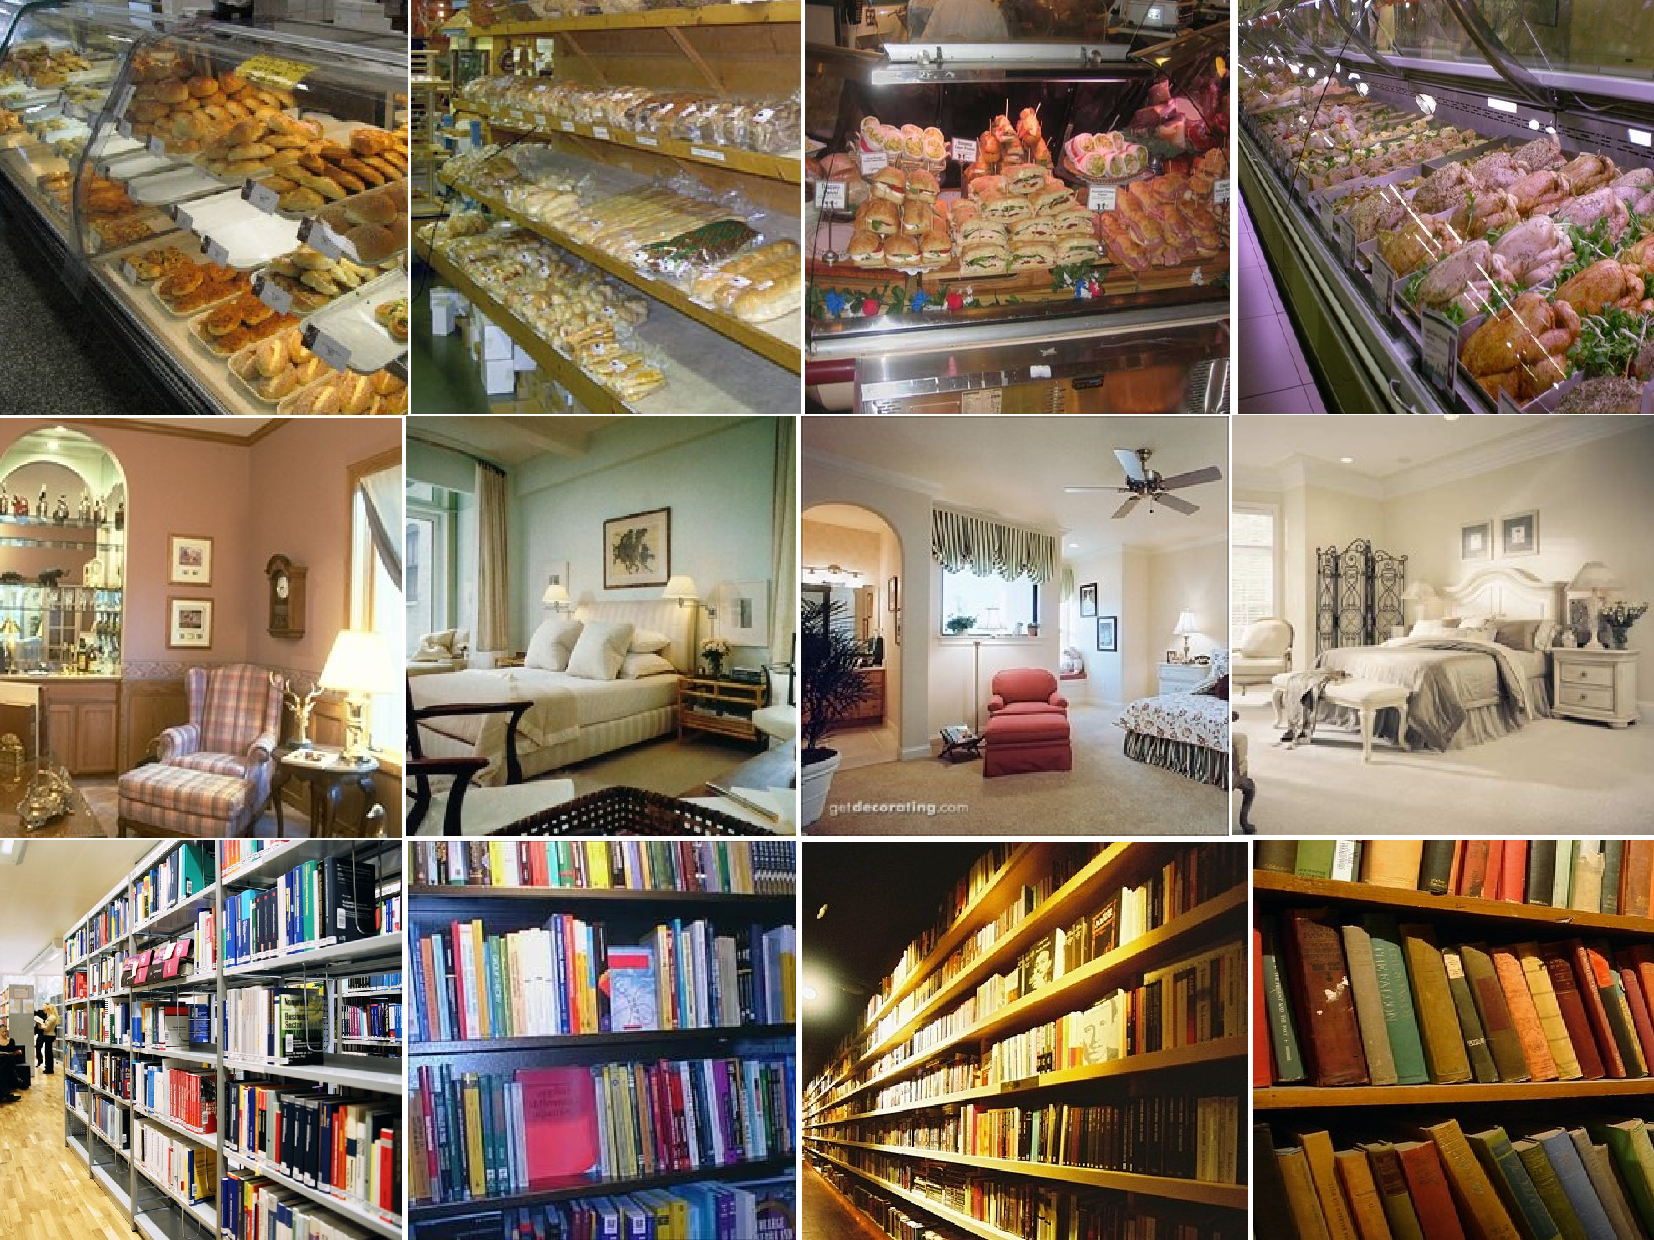
\includegraphics[width=0.45\textwidth]{img/dataset.pdf}
  \centering
  \caption{This figure contains some sample images from the MIT-indoor67 dataset.
For each row, left two columns are from the same category and right two columns are from
another. The first pair is bakery and deli, the second pair is living rooms and bedrooms, and the last pair is library and bookstore.}
\label{fig:sample}
\end{figure}

Multi-class classification is done with a 67 SVMs trained using one-versus-all rule, that is, each
classifier is learned to separate each class from the rest of classes. Test image is assigned the
label of the class with the highest confidence score. Scene classification performance is
evaluated by the average multi-class classification accuracy over all scene classes.

For comparison purpose, we implement with the same procedure but only use
the extracted layer 7 4096-dimensional feature vectors from Caffe. After we get
one feature vectors for each entire image, instead of perform spatial pyramid
and L2 normalization, we simply add labels and send them into the multi-class
SVMs. Validation image feature vectors are also generated in the same way.

% Table 1
\begin{table*}[ht]
        \caption{Comparison results on MIT-indoor67}
        \centering
        \begin{tabular}{l c c}
        \hline \hline
        Models                & Average Precision \\ \hline
        $l2$ Normlization + Selective Search + Spatial Pyramid & {\bf{68.2953\%}} \\
        Selective Search + Spatial Pyramid & 68.0469\% \\
        Entire Image CNN Features & 59.9507\% \\
        \hline
        \end{tabular}
        \label{tab:overall}
\end{table*}

\subsection{Quantitative Evaluation}
We compare our scene classification performance with two other methods: 1) using only the
features extracted from the entire image; 2) using selective search and spatial pyramid, but without the
$l2$ normalization. The summary of our performance comparison is listed in Table~\ref{tab:overall}.
Our method achieves a mean average precision (mAP) of 68.2953\% on dataset
MIT-indoor67. For comparison, we implement the same method using only 4096-dimensional
feature vectors extracted from Caffe without region proposals, spatial pyramid, and max-pooling.
Using selective search and spatial pyramid gives us a 8.1\% performance gain and introducing
the $l2$ normalization gives us an extra 0.25\% performance gain. In most categories, we perform much
better than the average precision. Some examples are shoes shop, bedroom, grocery store, hospital room and operating
room. We achieve 100\% precision on three categories: cloister, florist, and bowling. This is because the region proposals and spatial pyramid technique
allow us to better characterize the particular objects belong to the category. For those categories which achieve worst precision, the false positives are
not evenly distributed either, but are focused on some very sensible categories. For example the top two false positive categories for auditorium are concert hall
and movie theater.
We also note some drops of average accuracy using our methods. The drops mainly happen for on the following three categories: prison-cell, library and living room.
Note these three categories are all relatively easier to be characterized by global spatial properties (prison cell bars and books on shelves) so focusing on small regions
might suppress the representation of the global scene.

% top 5 best and top 5 worst table (Table 2)
\begin{table}[ht]
        \caption{Top 5 Best and Top 5 Worst Results}
        \centering
        \begin{tabular}{l l l}
        \hline \hline
        & Name           & Avg. Prec./Top FP Ctgr. \\ \hline
        \multirow{5}{*}{Top 5 Best}
        & cloister       & 100\% \\
        & florist        & 100\% \\
        & bowling        & 100\% \\
        & poolinside     & 95\% \\
        & greenhouse     & 94.74\% \\
        \hline
        \multirow{5}{*}{Top 5 Worst}
        & livingroom     & 20\%/bedroom \\
        & lobby          & 30\%/jelleryshop \\
        & deli           & 31.58\%/bakery \\
        & office         & 33.33\%/computer\_room \\
        & airport inside & 35\%/subway \\
        \hline
        \end{tabular}
        \label{tab:overall}
\end{table}

Table~\ref{tab:compare} compares the performance of our method against various other scene classification methods. Note that methods using CNNs all show significant improvements of the performance.
Also, our method which uses selective search and spatial pyramid achieves better performance than Zhou et al.'s work on both ImageNet-CNN and Places-CNN, a CNN trained on a dataset specific created for places.

% compare with other paper results
% Table 3
\begin{table}[ht]
        \caption{Comparison to other methods}
        \centering
        \begin{tabular}{l c c}
        \hline \hline
        Method                & Average Precision \\ \hline
        Object Bank~\protect\cite{Li:2010:OBA} & 37.6 \\
        DPM+GIST-color+SP~\protect\cite{Pandey:2011:SRW} & 43.1 \\
        ImageNet-CNN feature~\protect\cite{Zhou:2014:LDF} & 56.79 \\
        Places-CNN feature~\protect\cite{Zhou:2014:LDF} & 68.24 \\
        Our Method & 68.3 \\
        \hline
        \end{tabular}
        \label{tab:compare}
\end{table}

% heatmap visulizations
\subsection{Qualitative Evaluation}
\begin{figure}[ht]
  \centering
  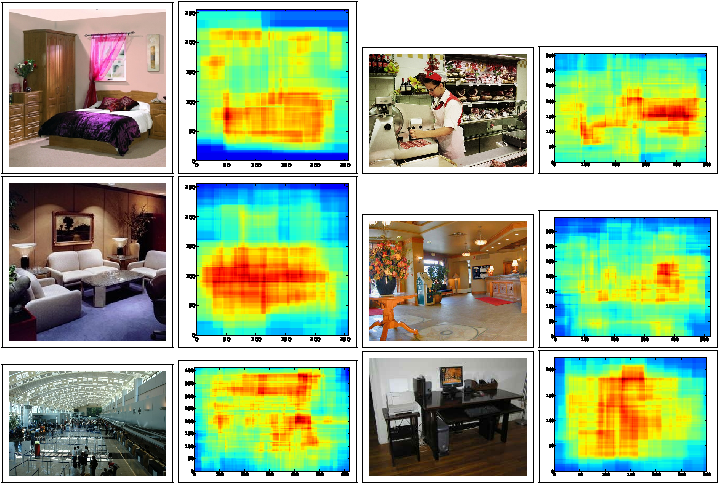
\includegraphics[width=0.45\textwidth]{img/tp.pdf}
  \centering
  \caption{True Positive Test examples. An example consists of the original test image (left) and the heatmap represented the highest response regions during the prediction (right). First row: bedroom (left) and deli (right); second row: livingroom (left) and lobby (right); and third row: airport\_inside (left) and office (right).}
  \label{fig:tp}
\end{figure}

For qualitative evaluation, we show samples of the true positive test examples in Figure~\ref{fig:tp}. Note that the selective search and spatial pryamid enable the algorithm to use the most informative region as the highest response during the prediction process. For example, in the bedroom example, highest responses are from bed and pollows; in the livingroom example, highest responses are from sofa and coffe table; and in the office example, desk and cabinet shelf. In large scenes, the highest responses are also focused around characteristic regions (airport\_inside's feature region is the glass ceiling and  the lobby's feature region is the checkin desk).

% heatmap visulizations
\begin{figure}[ht]
  \centering
  \includegraphics[width=0.45\textwidth]{img/fp.pdf}
  \centering
  \caption{False Positive Test examples. An example consists of the original test image (left) and the heatmap represented the highest response regions during the prediction (right). First row: lobby/airport\_inside (left) and subway/airport\_inside (right); second row: nursery/bedroom (left) and waitingroom/bedroom (right); third row: staircase/airport\_inside (left) and kindergarden/children\_room (right); forth row: bathroom/livingroom (left) and lockerroom/lobby (right); and fifth row: computerroom/office (left) and livingroom/office (right).}
  \label{fig:tp}
\end{figure}

The false positive test examples show some misclassification examples. The reasons are as follows: 1) Overfitting to the training sets. For example, airport inside which looks like a lobby or a subway station,  bedroom which looks like a nursery room, lobby which contains staircase in the scene, children room which contains too many toys that might appear more often in kindergarden category in the training set. 2) Wrong recognitions of key objects. For example in the bathroom/livingroom example recognizing the plate on the table as a hand washing sink, and in the lockerroom/lobby example recognizing the room doors as safe cases. 3) Failing the consider key objects. For example, in the waitingroom/bedroom example, the bed in the lower left corner is ignored by responses, and in the computerroom/office example, the desktop full of books and documents are also ignored. The false positive test examples show two places where we can improve the current model: First, a better method for extract regions of interest can be applied to increase the performance of selective search. Second, by carefully design better training dataset, the false positive cases will also be reduced.





